\documentclass[11pt,letterpaper]{article}

\usepackage[T1]{fontenc}
\usepackage[utf8]{inputenc}
\usepackage[expansion=false]{microtype}
\usepackage{geometry}
\usepackage{amsmath,amssymb}
\usepackage{fancyhdr}
\usepackage{titling}
\usepackage{listings}
\usepackage{xcolor}
\usepackage{url}
\usepackage{enumitem}
\usepackage{booktabs}
\usepackage{tabularx}
\usepackage{array}
\usepackage{graphicx}
\usepackage{float}
\usepackage{tikz}
\usepackage{needspace}
\usepackage[hidelinks]{hyperref}

\graphicspath{{results/figures/}}
% let pages carry more floats and pack float-only pages from the top,
% instead of leaving half-empty pages around each figure
\renewcommand{\topfraction}{0.9}
\renewcommand{\bottomfraction}{0.8}
\renewcommand{\textfraction}{0.07}
\renewcommand{\floatpagefraction}{0.85}
\setcounter{topnumber}{3}
\setcounter{bottomnumber}{2}
\setcounter{totalnumber}{5}
\makeatletter
\setlength{\@fptop}{0pt}
\setlength{\@fpsep}{14pt}
\makeatother
\setlist[enumerate]{itemsep=2pt, topsep=4pt, parsep=0pt, partopsep=0pt}
\setlist[itemize]{itemsep=2pt, topsep=2pt, parsep=0pt, partopsep=0pt}
\geometry{left=0.85in,right=0.85in,top=0.85in,bottom=0.85in}

\lstset{language=C, basicstyle=\ttfamily\footnotesize, columns=fullflexible,
  keepspaces=true, tabsize=4, xleftmargin=1.5em, aboveskip=6pt, belowskip=6pt,
  commentstyle=\color{black!60}}
\setlength{\emergencystretch}{3em} % long \texttt names can't hyphenate

\newcommand{\repo}{https://github.com/yazeed1s/tmalloc}
\newcommand{\src}[1]{\href{\repo/blob/main/#1}{\texttt{#1}}}

\title{CS 5204: Operating Systems \\ Individual Project: Midterm Checkpoint}
\author{Yazeed Alharthi \\ Sam H. Noh, Professor \\[4pt]
  \small Code: \url{https://github.com/yazeed1s/tmalloc}}
\date{October 29, 2026}

\pagestyle{fancy}
\fancyhf{}
\fancyhead[L]{CS 5204}
\fancyhead[C]{Midterm Checkpoint}
\fancyhead[R]{Yazeed Alharthi}
\fancyfoot[C]{\thepage}
\setlength{\headheight}{15pt}

\begin{document}

\maketitle

\begin{center}
  \rule{0.9\textwidth}{0.4pt}
\end{center}

\section{Where things stand}

The proposal promised three single-threaded allocators for this checkpoint, and all three are done: an implicit free list, an explicit free list and a segregated free list. They pass every test trace with a heap checker running after every single operation, they pass under AddressSanitizer, and I benchmarked all of them against glibc's \texttt{malloc} for speed and for memory.

I'm late on the schedule. The proposal had implicit done by October 4 and explicit by October 13, and that didn't happen; most of the work landed in the last stretch before this checkpoint. I built the phases in the planned order, just not on the planned dates. Everything after the midterm is still ahead of me: \texttt{calloc} and \texttt{realloc}, a global lock, per-thread caches, and running the allocator inside ZWM.

One thing changes how to read the numbers. Before the final runs I audited my own benchmark program and found a bug that made my allocators look much slower than they are on large heaps. Every number in this report is from after the fix. Section~\ref{sec:audit} explains the bug, and the old results are still in the repository under \texttt{results/checkpoint/}.

Sections~\ref{sec:background}--\ref{sec:versions} explain what an allocator does and how mine is built. Sections~\ref{sec:correct} and \ref{sec:measure} explain how I tested and measured it. Section~\ref{sec:results} has the results.

\section{What an allocator has to do}
\label{sec:background}

A program calls \texttt{malloc(n)} to get $n$ bytes and \texttt{free(p)} to give them back. The allocator owns one large region of memory, the \emph{heap}, and has to hand out pieces of it, called \emph{blocks}. It has to answer each request right away, without knowing what the program will ask for next, and it can never move a block once it has handed it out, because the program holds a pointer to it.

That leaves two things an allocator can be good or bad at.

\begin{itemize}
  \item Time. On every \texttt{malloc} it has to find a free block that is big enough. If it has to look at many blocks to find one, it is slow. I report this as throughput, millions of operations per second (Mops/s).
  \item Memory. Free memory can end up in pieces that are too small for the requests that come later, so the heap has to grow even though there is enough free memory in total. This is \emph{fragmentation}. I report it as \emph{peak utilization}: the most bytes the program had in use at one time, divided by the biggest the heap ever got. 1.0 would mean no waste at all.
\end{itemize}

These two pull against each other. Taking the first block that fits (\emph{first fit}) is quick but can waste memory. Looking for the block that fits best is slower but wastes less. Most of this report is about where each of my designs lands between the two.

A few more words come up again and again. When the chosen free block is bigger than the request, the allocator can \emph{split} it: give out the front part and keep the rest as a smaller free block. When a block is freed next to another free block, the allocator can \emph{coalesce} (merge) them into one bigger block, so that free memory doesn't break into ever smaller pieces. A \emph{free list} is a linked list of the free blocks, so the search doesn't have to look at blocks that are in use.

The term that matters most in this report is \emph{size class}. A size class is a range of block sizes that the allocator groups together, each with its own free list. Instead of searching one list that holds every free block, a request for 100~bytes looks only in the list for, say, 64--128-byte blocks. How the classes are chosen decides a lot about both costs:
\begin{itemize}
  \item Wide classes (few lists) mix many sizes in each list, so the search can still walk past blocks that are too small, and the lists get long in big programs.
  \item Narrow classes (many lists) mean almost every block in a list fits, so the search is short, at the price of more lists to keep track of.
  \item Some allocators round every request up to the top of its class, which makes reuse easy but wastes the extra bytes. Mine doesn't round up: it splits blocks to the exact size, so its classes only affect how long the search takes and which block it picks.
\end{itemize}
My implicit and explicit versions have no classes at all. The segregated version uses 11: one per power of two from 32~bytes to 32~KiB, plus one for everything larger (Section~\ref{sec:versions}). glibc's are much finer, 16~bytes apart for small sizes. Most of the differences in Section~\ref{sec:results} come back to this choice.

The baseline is glibc 2.44's \texttt{malloc}, which is what nearly every Linux program uses. It is a lot more than a free list. Recently freed small blocks go into per-thread caches (\emph{tcache}) and \emph{fastbins}, where they are reused as they are, without splitting or merging. Small blocks are sorted into \emph{bins} (glibc's name for size classes) 16~bytes apart, so finding a small block needs no search. Large free blocks sit in bins sorted by size. Requests above 128~KiB skip the heap entirely: glibc gets them straight from the kernel with \texttt{mmap} and returns them with \texttt{munmap} on free. Several of my results come back to one of these features.

\section{How the code is organized}
\label{sec:code}

The whole project is in the repository linked at the top, about 2,100 lines of C plus Python for the traces and plots.

\begin{center}
\footnotesize
\begin{tabularx}{\textwidth}{@{}l r X@{}}
\toprule
file & lines & what it is \\
\midrule
\src{src/tmalloc.h} & 61 & the interface every allocator version implements \\
\src{src/memlib.c} & 129 & hands the allocator raw memory to build its heap in \\
\src{src/implicit.c} & 291 & version 1, implicit free list \\
\src{src/explicit.c} & 357 & version 2, explicit free list \\
\src{src/segregated.c} & 413 & version 3, segregated free lists (and the seg-skip variant) \\
\src{src/glibc.c} & 96 & wraps glibc's \texttt{malloc} in the same interface, so it can be benchmarked the same way \\
\src{bench/driver.c} & 722 & the benchmark: replays a trace against one allocator and measures it \\
\texttt{tools/} & & trace generator, plots, the independent memory check, the benchmark scripts \\
\texttt{tests/} & & tests for \texttt{memlib} and for the heap checker \\
\bottomrule
\end{tabularx}
\end{center}

The decision that shapes everything else is that all versions share one interface:

\begin{lstlisting}
int    tmm_init(void);          /* set up (or reset) the heap */
void  *tmm_malloc(size_t size);
void   tmm_free(void *ptr);
int    tmm_check(void);         /* walk the heap, 0 if everything is consistent */
tmm_stats_t tmm_get_stats(void);/* blocks searched, splits, merges, heap growths */
\end{lstlisting}

The functions are prefixed \texttt{tmm\_} so they don't replace the real \texttt{malloc} that the rest of the program (and the C library) still uses. Because the interface is the same, the Makefile builds the same benchmark program once per allocator: \texttt{bench\_implicit}, \texttt{bench\_explicit}, \texttt{bench\_segregated}, \texttt{bench\_segregated-skip} and \texttt{bench\_glibc}. Adding a new version means adding one file to \texttt{src/}. Every allocator runs through exactly the same benchmark code, which is what makes the comparison fair.

The statistics are there to explain the timing. If a version is slow on some trace, I can look at how many blocks its \texttt{malloc} searched or how many times it split a block, and usually the reason is right there.

\section{What every version shares}
\label{sec:shared}

\subsection*{Where the heap memory comes from}

The heap comes from \src{src/memlib.c}, which works like the old Unix \texttt{sbrk}: one region with an end pointer (the \emph{break}) that I move forward when I need more space. At startup it reserves 4~GiB of addresses with one \texttt{mmap} (\texttt{PROT\_NONE}, \texttt{MAP\_NORESERVE}), which costs no physical memory, and \texttt{tmm\_sbrk(n)} moves the break and calls \texttt{mprotect} on the new pages. So the heap is one contiguous range (merging never hits a gap), every growth is a system call I can count, which is the OS side of this project, and untouched pages cost nothing. It grows by at least 64~KiB at a time, just my first guess between too many system calls and too much unused heap.

\subsection*{What a block looks like}

Each block has an 8-byte \emph{header} and an 8-byte \emph{footer}, both holding the block's size and an allocated bit (sizes are multiples of 16, so a low bit is free for that). The \emph{payload} the program gets comes right after the header, 16-byte aligned like C requires. A free block keeps \texttt{next} and \texttt{prev} pointers in its unused payload, so the smallest block is 32~bytes.

\begin{center}
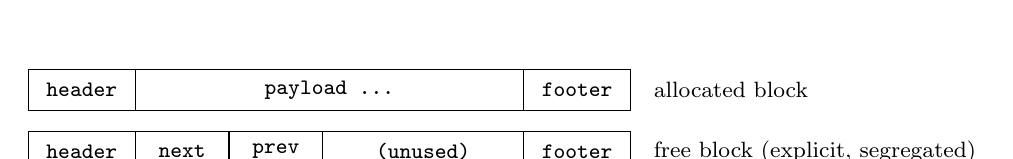
\begin{tikzpicture}[x=0.85cm,y=0.65cm, every node/.style={font=\footnotesize\ttfamily}]
  \draw (0,1.2) rectangle (1.6,2) node[midway] {header};
  \draw (1.6,1.2) rectangle (7.4,2) node[midway] {payload ...};
  \draw (7.4,1.2) rectangle (9,2) node[midway] {footer};
  \node[anchor=west] at (9.2,1.6) {\rmfamily allocated block};
  \draw (0,0) rectangle (1.6,0.8) node[midway] {header};
  \draw (1.6,0) rectangle (3.0,0.8) node[midway] {next};
  \draw (3.0,0) rectangle (4.4,0.8) node[midway] {prev};
  \draw (4.4,0) rectangle (7.4,0.8) node[midway] {(unused)};
  \draw (7.4,0) rectangle (9,0.8) node[midway] {footer};
  \node[anchor=west] at (9.2,0.4) {\rmfamily free block (explicit, segregated)};
\end{tikzpicture}
\end{center}

The header lets me step to the next block (address plus size). The footer is for going backwards: when a block is freed I read the word just before its header, the previous block's footer, and know right away if that neighbour is free and how big. Without it, merging backwards would mean walking the heap from the start. A \emph{prologue} block and an \emph{epilogue} header, always marked allocated, mean the merge code never has to check for the heap's edges.

\subsection*{The path of a request}

\texttt{tmm\_malloc} is almost the same in every version:

\begin{lstlisting}
size_t asize = MAX(ALIGN(size + DSIZE), MIN_BLOCK); /* add header+footer, round to 16 */
char  *bp    = find_fit(asize);                     /* the part each version does differently */
if (bp == NULL)
	bp = extend_heap(MAX(asize, CHUNKSIZE));        /* nothing fits: grow by >= 64 KiB */
place(bp, asize);                                   /* mark allocated, split if worth it */
\end{lstlisting}

\texttt{place} splits only if the leftover is at least 32~bytes, and \texttt{tmm\_free} merges the block with any free neighbours in constant time. Every version splits down to exactly the rounded size, so the versions only differ in how \texttt{find\_fit} searches and where freed blocks are kept.

\section{Three versions, each fixing the last one's problem}
\label{sec:versions}

\subsection*{Version 1: implicit free list}

The simplest search walks every block in address order and takes the first free one that's big enough:

\begin{lstlisting}
for (char *bp = NEXT_BLKP(heap_listp); GET_SIZE(HDRP(bp)) > 0; bp = NEXT_BLKP(bp))
	if (!GET_ALLOC(HDRP(bp)) && GET_SIZE(HDRP(bp)) >= asize)
		return bp;
\end{lstlisting}

It's ``implicit'' because there's no real list, the sizes link the blocks. It packs memory well, but it also steps over every \emph{allocated} block, so it gets slower as the whole heap grows.

\subsection*{Version 2: explicit free list}

So next I kept only the free blocks in a doubly linked list, through the pointers in their payloads. The search is the same loop over the list instead of the heap. Doubly linked so I can remove a block from the middle in constant time when a neighbour merges. A freed block goes to the front (LIFO), which is constant time. An address-sorted list usually fragments less but makes every \texttt{free} walk the list, I went with the fast one first to see what it costs (Section~\ref{sec:r-search}).

\subsection*{Version 3: segregated free lists}

One list still mixes all sizes, so a 2~KiB request can walk past lots of small blocks. The fix is size classes (Section~\ref{sec:background}). I have 11: one per power of two from $[32,64)$ to $[16\text{K},32\text{K})$, plus one for everything bigger, and a bitmap of non-empty lists so finding the next one is a single \texttt{\_\_builtin\_ctz}.

A request's own class can hold blocks that are too small (a 48-byte request is in $[32,64)$, which may only have 32-byte blocks), so should the search look there at all? I built both answers. Option (a), the default, searches its own class with first fit and otherwise takes the first block of the next non-empty larger class:

\needspace{8\baselineskip}
\begin{lstlisting}
int c = size_class(asize);
for (free_node_t *n = free_heads[c]; n; n = n->next)   /* (a): search own class */
	if (GET_SIZE(HDRP(n)) >= asize)
		return n;
uint32_t larger = nonempty & ~((2u << c) - 1);         /* non-empty classes above c */
return larger ? free_heads[__builtin_ctz(larger)] : NULL;
\end{lstlisting}

Option (b), \emph{seg-skip}, skips its own class, so every search is one step but it often splits a bigger block than needed (same file, one compile flag). I added it when my first results showed (a) searching \emph{more} blocks than explicit on some traces. I assumed powers of two would be fine enough, Section~\ref{sec:r-scale} shows where that stopped being true.

\section{How I know it's correct}
\label{sec:correct}

A broken allocator usually doesn't crash right away. It hands out two overlapping blocks or loses a free one, and the program fails much later somewhere unrelated. So I wanted bugs caught at the operation that caused them.

Each version has a heap checker, \texttt{tmm\_check()}. It first walks the heap and checks every block (header matches footer, aligned, inside the heap, no two free blocks next to each other). Then it walks the free lists and checks they agree with the heap: every listed block is really free, \texttt{prev} and \texttt{next} agree, each block is in the right class, the bitmap matches, and the free-block counts are the same. A checker that always says ``ok'' looks exactly like a working one, so \src{tests/check\_test.c} corrupts the heap in six ways and makes sure each one is caught, for every version. The benchmark also writes a pattern unique to each block into its payload and checks it before \texttt{free}, so overlapping blocks would show up. I tested that against a broken allocator that returns the same buffer every time, and it caught it.

Every trace passes with the checker running after every single operation, in the normal build and under AddressSanitizer.

\section{How I measured it}
\label{sec:measure}

\subsection*{Traces}

The benchmark replays \emph{traces}: text files with one operation per line, \texttt{a 17 512} meaning ``allocate 512 bytes as block 17'' and \texttt{f 17} meaning ``free block 17''. A Python script (\texttt{tools/gentrace.py}) generates them from fixed random seeds, so every allocator sees exactly the same sequence on any machine. Every trace frees everything it allocates.

There are two groups. The \emph{main suite} keeps every request under 128~KiB. Above that size glibc doesn't use its heap at all (it calls \texttt{mmap} directly), and mine has no such path yet, so leaving large sizes out makes the main suite a fair test of the free-list designs. The \emph{stress suite} has no limits; its job is to find where my allocators break and why.

\begin{center}
\footnotesize
\begin{tabularx}{\textwidth}{@{}lX@{}}
\toprule
trace & what it does \\
\midrule
\multicolumn{2}{@{}l}{\emph{main suite}} \\
\texttt{small-fixed} & 16--64~B, about 1000 live, 100k ops, the easy case \\
\texttt{random} & uniform 1~B--4~KiB, random free order, 100k ops \\
\texttt{bimodal} & 90\% 8--64~B, 10\% 4--64~KiB, 100k ops, fragmentation stress \\
\texttt{throughput} & 16~B--1~KiB, about 1000 live, 1M ops \\
\texttt{grow-free-all} & 4 rounds of: allocate 5000 blocks, free them all \\
\texttt{checkerboard} & alternate 32/512~B, free the 32s, then ask for 256~B (holes too small to reuse) \\
\midrule
\multicolumn{2}{@{}l}{\emph{stress suite}} \\
\texttt{scale-1k} \ldots\ \texttt{128k} & random 1~B--4~KiB with \emph{exactly} 1k, 2k \ldots\ 128k blocks live, 500k steady-state ops each \\
\texttt{holes-1k} \ldots\ \texttt{16k} & $N$ free 32~B holes that can't merge, then $2000\times 1$~KiB requests \\
\texttt{large-holes-500} \ldots\ \texttt{8000} & $N$ free 40~KiB holes that can't merge, then $500\times 100$~KiB requests none of them can serve \\
\texttt{huge-churn} & 128~KiB--4~MiB blocks, about 64 live \\
\texttt{recycle-}$S$\texttt{-pinned/-freed} & 1000 blocks of one size $S$ (32 \ldots\ 1024~B, or mixed) freed and reallocated 200k times, a controlled pair \\
\texttt{dist-*}, \texttt{frag-grow} & the same 2000-live churn under five size distributions, and growing sizes that strand their holes \\
\bottomrule
\end{tabularx}
\end{center}

I skipped implicit on the scale traces from 8k live blocks up. At 4k it already searches 2770 blocks per \texttt{malloc}, so each of those runs would take minutes to show what is already clear: it gets slower in proportion to the heap.

\subsection*{The benchmark program}

\src{bench/driver.c} runs each trace in three separate passes, so that measuring one thing doesn't disturb another. An untimed memory pass tracks live bytes and heap size and checks the payload patterns. A timing pass does a warm-up and then up to ten runs that only call \texttt{malloc} and \texttt{free}, and I report the median. A counter pass uses \texttt{perf\_event\_open} to count cycles, instructions, L1 cache misses and dTLB misses (the CPU had to look up where a page physically lives) per operation, in user space only.

Besides utilization, I measured resident memory (RSS, the physical memory actually used) and checked it a second time from outside the process. The two agree within 4\% above 4~MB.

\subsection*{The bug I found in my own benchmark}
\label{sec:audit}

Before the final runs I went through the driver looking for anything that favoured one allocator. The serious problem: \texttt{tmm\_init()} reset my heap between timed runs by mapping fresh memory over it, so every run of mine faulted the whole heap back in while glibc's heap stayed warm. On \texttt{scale-64k} that was about 20,800 page faults per run, exactly its 83~MB heap in 4~KiB pages. The reset now keeps the pages. Two smaller fixes: the driver's own arrays had been counted in glibc's heap, and its \texttt{/proc} reads called \texttt{malloc}.

\begin{center}
\footnotesize
\begin{tabular}{@{}l r r@{}}
\toprule
 & before fix & after fix \\
\midrule
explicit, main suite (geometric mean vs glibc) & 0.52$\times$ & 1.09$\times$ \\
seg-skip at 64k live blocks (vs glibc) & 0.31$\times$ & 0.81$\times$ \\
\texttt{large-holes-8000}, explicit (vs glibc) & 0.06$\times$ & 0.20$\times$ \\
\texttt{huge-churn}, explicit (vs glibc) & 1.58$\times$ & 78$\times$ \\
\bottomrule
\end{tabular}
\end{center}

glibc's numbers didn't move. Two of my earlier conclusions came from the bad numbers (explicit at half of glibc's speed, seg-skip slowed by cache misses), and I dropped both. One limitation remains: the timed loop never writes into its blocks, which hides the cost of touching fresh memory.

\subsection*{Keeping the machine quiet}

My first timings swung by up to 1.87$\times$ on the same trace, because of background apps and the power manager toggling CPU boost. The final numbers come from \texttt{quiet-bench.sh}, which fixes the CPU frequency with boost off, pins the benchmark to one core, and runs everything three times (AMD Ryzen 7 PRO 6850U, Linux 6.18, glibc 2.44, gcc 16.2, \texttt{-O2}). Even so, 28 of 215 allocator/trace pairs still vary by more than 10\% between rounds, for a reason I couldn't pin down. So every speed is a median of three rounds, I only claim a win if it holds in each round, and noisy results are marked.

\section{Results}
\label{sec:results}

Short version: once I fixed the search, my explicit list got pretty close to glibc, 1.09$\times$ its speed on average over the main suite. But that average is kind of misleading, on one trace I'm 3.2$\times$ faster and on another less than half as fast. Most of this section is me trying to figure out why.

Some terms first. ``Speed vs glibc'' is my speed divided by glibc's, so above 1 means I'm faster. ``Utilization'' is how much of the heap actually holds the program's data at its peak (1.0 means nothing wasted). ``Blocks searched'' is how many free blocks \texttt{malloc} looked at before finding one that fits.

\subsection{How do my allocators compare?}
\label{sec:r-search}

\begin{figure}[H]
  \centering
  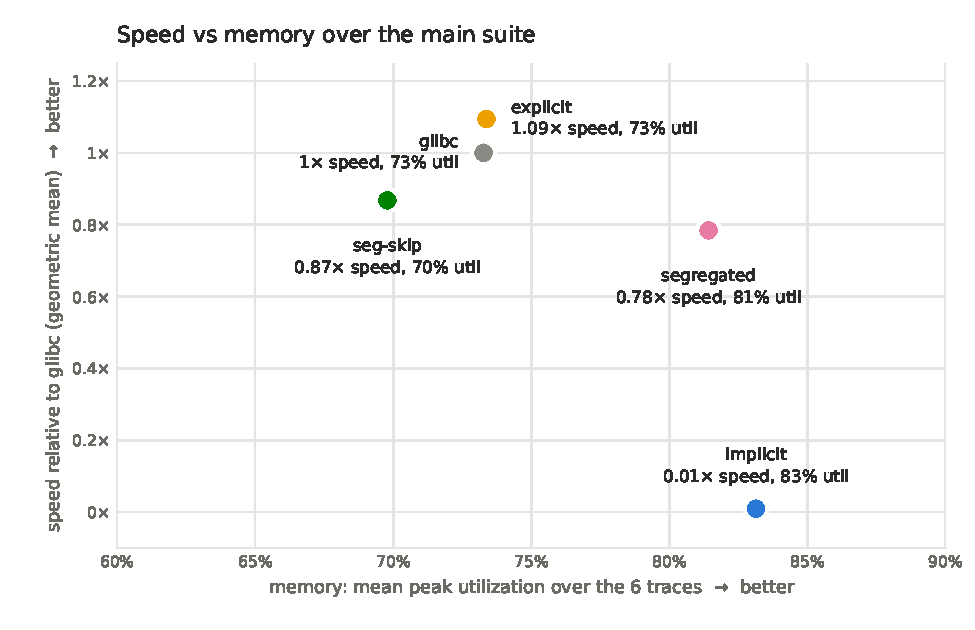
\includegraphics[width=0.5\textwidth]{tradeoff.pdf}
  \caption{Main suite: speed relative to glibc (geometric mean over the six traces) against average peak utilization. Up is faster, right wastes less memory.}
  \label{fig:tradeoff}
\end{figure}

\begin{table}[H]
\centering
\footnotesize
\begin{tabular}{@{}l r r r r r@{\hspace{2.2em}}r r r r@{\hspace{2.2em}}r r r r r@{}}
\toprule
 & \multicolumn{4}{c}{speed vs glibc} & \multicolumn{4}{c}{blocks searched / malloc} & \multicolumn{5}{c}{peak utilization} \\
 & impl & expl & seg & skip & impl & expl & seg & skip & glibc & impl & expl & seg & skip \\
\midrule
small-fixed   & 0.028 & 0.65 & 0.62 & 0.46 & 344 & 1.9 & 2.2 & 1.0 & 0.25 & 0.52 & 0.52 & 0.52 & 0.26 \\
random        & 0.022 & 1.66 & 0.79 & 1.59 & 815 & 4.3 & 14.7 & 1.0 & 0.85 & 0.90 & 0.78 & 0.88 & 0.69 \\
bimodal       & 0.027 & 0.77 & 0.85 & 0.73 & 611 & 3.7 & 3.6 & 1.1 & 0.87 & 0.87 & 0.47 & 0.78 & 0.72 \\
throughput    & 0.009 & 0.45 & 0.25 & 0.37 & 524 & 2.8 & 10.5 & 1.0 & 0.58 & 0.83 & 0.75 & 0.83 & 0.64 \\
grow-free-all & 0.006 & 3.19 & 1.97 & 1.89$^\ast$ & 2500 & 1.0 & 1.0 & 1.0 & 0.96 & 0.97 & 0.97 & 0.97 & 0.97 \\
checkerboard  & 0.0007 & 1.47 & 1.15 & 1.14 & 7500 & 4.8 & 1.0 & 1.0 & 0.88 & 0.90 & 0.90 & 0.90 & 0.90 \\
\bottomrule
\end{tabular}
\caption{The main suite, median of 3 rounds. glibc's own speeds: 82, 19, 46, 89, 22 and 37~Mops/s in the order above. $^\ast$rounds differ by more than 10\% (1.52--1.94).}
\label{tab:results}
\end{table}

I expected blocks searched to explain most of the speed (Table~\ref{tab:results}), and it mostly does. Implicit walks every block in the heap, free or not, so it is 36$\times$ to 1350$\times$ slower than glibc. That was expected, it's why I built the other versions. It does have the best memory use of mine though, since it only grows the heap when nothing fits anywhere.

Explicit searches only 1 to 5 blocks, and then the traces split into two groups, the same way every round. I'm faster than glibc on \texttt{random}, \texttt{checkerboard} and \texttt{grow-free-all} (1.47--3.19$\times$) and slower on the small-object traces (0.45--0.77$\times$). My guess for small objects is glibc's tcache and fastbins, small per-size caches where a freed block just waits and is handed back on the next \texttt{malloc} of that size, no splitting or merging. Mine always merges a freed block with its neighbours and splits it again later. I test this in Section~\ref{sec:r-break}. Why glibc is so slow on \texttt{grow-free-all} I don't really know, it runs about 3$\times$ my instructions per operation but I couldn't tell which part of glibc that is.

Explicit pays for the speed in memory, on \texttt{bimodal} it wastes more than half the heap (0.47). I think it's the LIFO choice: a freed big block goes to the front of the list, small requests cut pieces off it, and when the next big request comes nothing big is left so the heap grows. An address-ordered list would probably fix that but makes \texttt{free} slower.

Segregated gets most of that memory back (0.78) because it only searches blocks of about the right size, a bit like best fit. But it's slower than explicit, since its class is full of blocks just slightly too small that it has to walk past (14.7 per \texttt{malloc} on \texttt{random} vs 4.3). Seg-skip looks at exactly one block but splits bigger blocks for small requests, so it wastes the most. So picking a block more carefully saves memory and costs time, and none of my versions got both. glibc avoids this for small sizes with bins 16~bytes apart where every block in a bin fits, which is probably where I need to go.

\subsection{What happens as the heap grows?}
\label{sec:r-scale}

The main suite keeps only about a thousand blocks live, which is small for a real program. So I ran the same random workload with exactly 1k, 2k, up to 128k blocks live (Figure~\ref{fig:scaling}).

\begin{figure}[H]
  \centering
  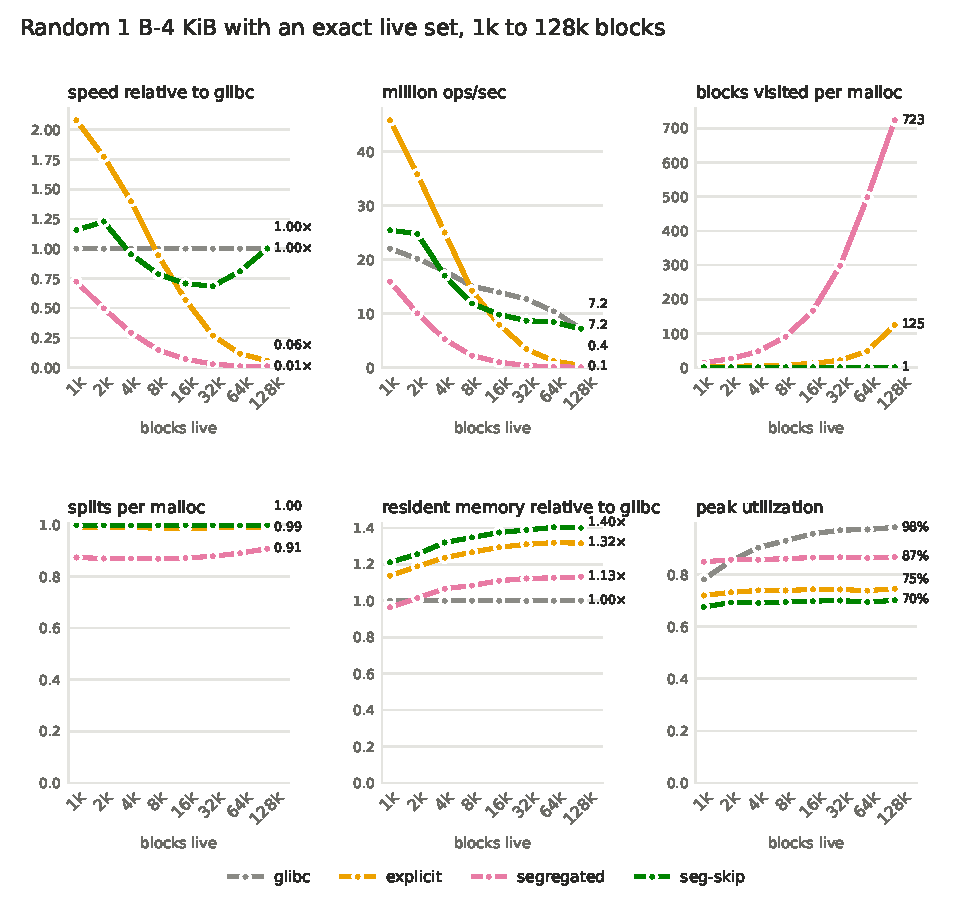
\includegraphics[width=0.495\textwidth]{scaling.pdf}\hfill
  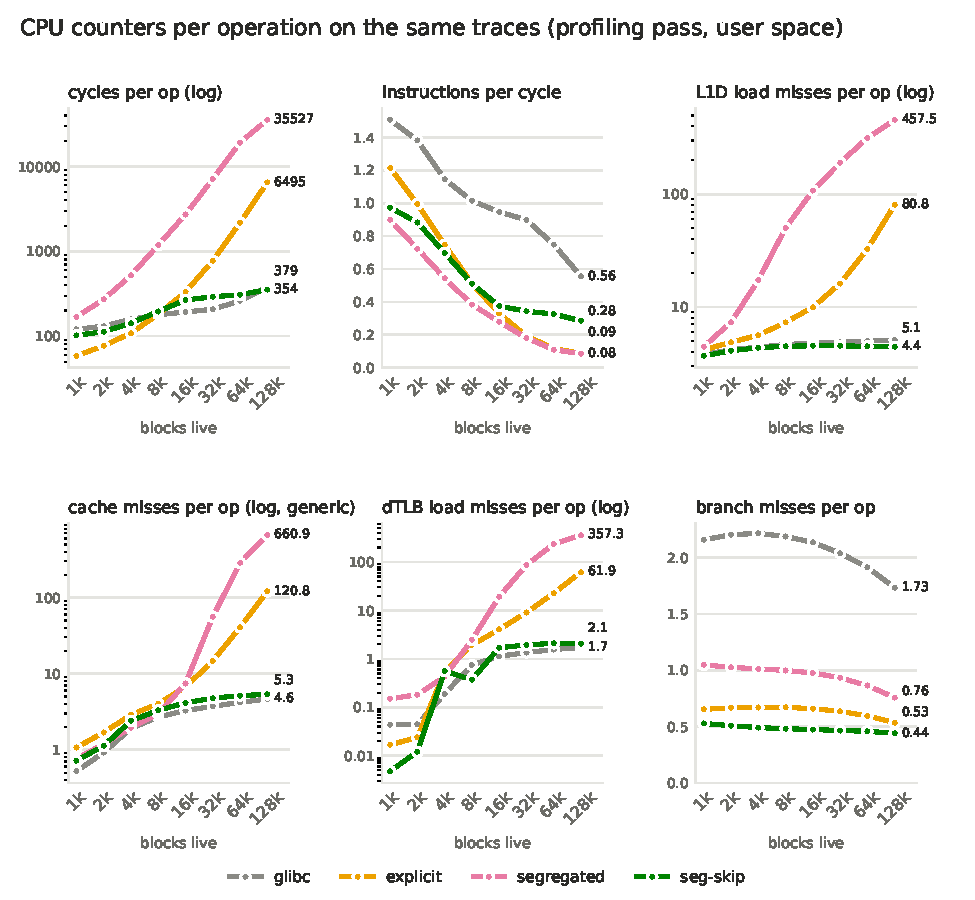
\includegraphics[width=0.495\textwidth]{hardware.pdf}
  \caption{Random 1~B--4~KiB with 1k to 128k blocks live. Left: speed vs glibc, absolute speed, blocks searched per \texttt{malloc}, splits per \texttt{malloc}, resident memory vs glibc, peak utilization. Right: CPU counters per operation (user space only, count panels on a log scale).}
  \label{fig:scaling}
  \label{fig:hardware}
\end{figure}

This is where it goes bad for me. Explicit is 2.08$\times$ faster than glibc at 1k, glibc catches up between 4k and 8k, and at 128k I'm about 17$\times$ slower. The search comes back: the list gets longer and explicit goes from 2.6 blocks per \texttt{malloc} to 125. Segregated is worse, 15 to 723. I thought the classes would protect it, but a class like $[2\text{K},4\text{K})$ just fills up with thousands of blocks and searching inside it is still a linear walk. I didn't expect that to break this early. Seg-skip, which always searches one block, stays close to glibc at every size (0.68--1.23$\times$, noisy).

But 125 blocks isn't that many, so why is it so slow? The right side of Figure~\ref{fig:scaling} has the CPU counters. An L1 miss means the data wasn't in the CPU's smallest, fastest cache, and a dTLB miss means the CPU also had to look up where the address is in physical memory, both are slow. For explicit, cycles per operation go up about 100$\times$ and the misses go up with them. My guess is that each step of the walk jumps to a random spot in a 100~MB heap so almost every step misses. I never changed only the walk length though, so it's a correlation, not a proof.

Memory gets worse too. glibc's utilization goes from 78\% to 98\% as the heap grows and mine stays flat, at 128k I use 1.13--1.40$\times$ glibc's physical memory. Not sure why glibc improves, maybe its finer bins fit better when there's more blocks to pick from, I haven't looked.

\subsection{Where does performance break down?}
\label{sec:r-break}
\label{sec:r-recycle}

Besides big heaps I found three more cases where I fall behind, or where the comparison isn't fair.

\paragraph{Small objects of a few sizes.} In Section~\ref{sec:r-search} I guessed glibc wins here because it reuses a freed block as is, so I tried to test only that. Each \texttt{recycle} trace keeps 1000 blocks of one size live and frees and reallocates them 200k times. In the \emph{pinned} version a 32-byte block that is never freed sits after every block, so nothing can merge and the next \texttt{malloc} gets its block back whole. In the \emph{freed} version those small blocks are freed first, so blocks merge and have to be split again.

\begin{figure}[H]
  \centering
  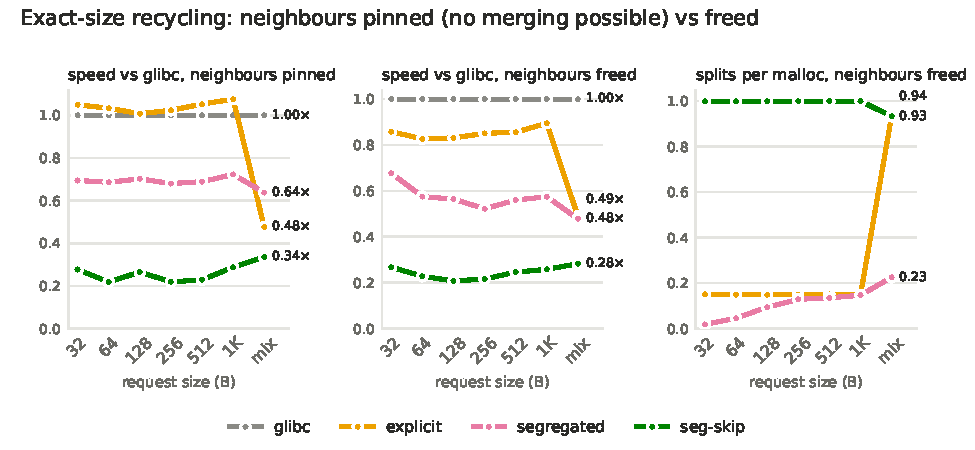
\includegraphics[width=0.85\textwidth]{recycle.pdf}
  \caption{Speed relative to glibc with neighbours pinned (left) and freed (middle), and splits per \texttt{malloc} with them freed (right).}
  \label{fig:recycle}
\end{figure}

glibc doesn't care either way (0.98--1.01), so it works as a control. Explicit gets 1.20--1.24$\times$ faster when it can't merge, at every size and every round, and that puts it level with glibc (Figure~\ref{fig:recycle}). So I think my guess was right, at least here. Pinning also shifts the layout a bit, so I can't say exactly what the merge itself costs. Seg-skip was really bad (0.21--0.34$\times$): it never looks in the request's own class, so even with an exact fit sitting there it splits a bigger block. I hadn't noticed that before, its a real flaw.

To see if this matters outside my made-up trace I ran the random workload with other size distributions (Table~\ref{tab:dist}).

\begin{table}[H]
\centering
\footnotesize
\begin{tabular}{@{}l r r r r l@{}}
\toprule
trace & explicit & segregated & seg-skip & glibc Mops/s & fastest \\
\midrule
\texttt{random} (uniform) & 1.66$\times$ & 0.79$\times$ & 1.59$\times$ & 19.1 & explicit \\
\texttt{dist-bimodal}     & 1.05$\times$ & 0.56$\times$ & 0.93$\times$ & 36.8 & explicit \\
\texttt{dist-loguniform}  & 1.29$\times$ & 0.62$\times$ & 0.91$\times$ & 27.0 & explicit \\
\texttt{dist-boundary}    & 0.91$\times$ & 0.39$\times$ & 0.80$\times$ & 39.2 & glibc \\
\texttt{dist-small}       & 0.49$\times$ & 0.42$\times$ & 0.34$\times$ & 120.7 & glibc \\
\texttt{dist-classes}     & 0.44$\times$ & 0.22$\times$ & 0.31$\times$ & 98.5 & glibc \\
\texttt{frag-grow}        & 0.27$\times$ & 0.01$\times$ & 1.60$\times$ & 27.0 & seg-skip \\
\bottomrule
\end{tabular}
\caption{Speed relative to glibc under different size distributions. The ``fastest'' column is the same in all three rounds.}
\label{tab:dist}
\end{table}

Explicit wins when sizes are spread out and glibc wins by about 2$\times$ on mostly small objects or a few fixed sizes. I'd guess real programs look more like the second case (lots of small structs and strings), so my uniform trace probably makes me look better than I am. Sizes right at my class edges (\texttt{dist-boundary}) raised segregated's search less than I expected, so I think long lists matter more than awkward sizes.

\paragraph{Free blocks that don't fit.} Here the heap is full of holes too small for the next request (Table~\ref{tab:stress}). With small holes I expected explicit to walk all of them, but it only searched 9--17. The leftover piece of the first split goes to the front of the list (LIFO again) and the next request finds it right away. It still drops to 0.43$\times$ glibc at 16k holes. Segregated never sees these holes, they're in another class, so it stays ahead of glibc.

\begin{table}[H]
\centering
\footnotesize
\begin{tabular}{@{}l r r r r@{}}
\toprule
trace & glibc Mops/s & explicit & segregated & blocks searched \\
 & & (vs glibc) & (vs glibc) & per request \\
\midrule
\texttt{holes-1k}  & 38.2 & 1.47$\times$ & 1.72$\times$ & 9 / 1 \\
\texttt{holes-4k}  & 41.3 & 0.79$\times^\ast$ & 1.24$\times$ & 14 / 1 \\
\texttt{holes-16k} & 40.5 & 0.43$\times^\ast$ & 1.10$\times$ & 17 / 1 \\
\midrule
\texttt{large-holes-500}  & 2.1 & 2.72$\times$ & 2.53$\times$ & $\approx$500 \\
\texttt{large-holes-2000} & 6.8 & 0.32$\times$ & 0.45$\times$ & $\approx$2000 \\
\texttt{large-holes-8000} & 6.7 & 0.20$\times$ & 0.20$\times$ & $\approx$8000 \\
\midrule
\texttt{huge-churn} & 0.56 & 78$\times$ & 51$\times$ & 2 \\
\bottomrule
\end{tabular}
\caption{Holes and big blocks. Last column: explicit / segregated per \texttt{malloc} for \texttt{holes}, per 100~KiB request for \texttt{large-holes} (the same for both). $^\ast$noisy: rounds 0.77--0.95 and 0.39--0.82.}
\label{tab:stress}
\end{table}

Large holes are where my design really breaks. Every 100~KiB request walks all $N$ of the 40~KiB holes and none fit. LIFO doesn't help because the heap grows by only 64~KiB so there's no leftover piece, and segregated doesn't help because everything over 32~KiB is in one class. At 500 holes I'm 2.7$\times$ faster than glibc, at 8000 5$\times$ slower and still getting worse. glibc's large bins are sorted by size with links that skip to the next size (dlmalloc uses a tree), mine is one unsorted list. \texttt{frag-grow} is the same problem for segregated, 2248 blocks per \texttt{malloc}.

\paragraph{Huge blocks.} For 128~KiB to 4~MiB I'm 51--78$\times$ faster, but I don't think that's fair. glibc gets each huge block from the kernel with \texttt{mmap} and returns it with \texttt{munmap}, two system calls per block, while my heap reuses what it has and never gives it back (11\% more physical memory). My benchmark also never writes into the blocks, so touching new pages isn't measured. I need my own \texttt{mmap} path before this means much.

\subsection{What did I learn?}
\label{sec:r-learned}

\begin{table}[H]
\centering
\footnotesize
\begin{tabularx}{\textwidth}{@{}>{\raggedright\arraybackslash}X >{\raggedright\arraybackslash}X >{\raggedright\arraybackslash}X@{}}
\toprule
where & result & my explanation \\
\midrule
\multicolumn{3}{@{}l}{\emph{mine loses}} \\
many live blocks (8k and up) & explicit 17$\times$, segregated 95$\times$ slower at 128k & long free-list walks, probably a cache miss on each step \\
small objects, a few fixed sizes & about 2$\times$ slower & I merge and re-split where glibc reuses blocks as they are \\
many large free blocks & 3--5$\times$ slower, growing & one unsorted list for every block over 32~KiB \\
memory at large heaps & 13--40\% more physical memory & glibc packs better as the heap grows, mine stays flat \\
\midrule
\multicolumn{3}{@{}l}{\emph{mine wins}} \\
small to medium heaps, spread-out sizes & explicit up to 2$\times$ faster & the free list stays short \\
allocate everything, then free everything & 3.2$\times$ faster & not sure, glibc runs about 3$\times$ the instructions \\
many small holes (segregated) & 1.1--1.7$\times$ faster & the holes are in a different class \\
\bottomrule
\end{tabularx}
\caption{Summary of where my allocators win and lose against glibc.}
\label{tab:summary}
\end{table}

The main thing I learned is that fixing the search once wasn't enough. Almost every loss in Table~\ref{tab:summary} is a search or a merge that glibc doesn't do at all, and my wins are mostly cases where my list happens to stay short. That's less impressive than I thought when I first saw the 1.09$\times$.

There's a lot these results don't show. All traces are synthetic and single-threaded, so I don't know yet how this looks with threads or a real program. 28 of 215 allocator/trace pairs still vary more than 10\% between rounds and I couldn't figure out why. The cache explanation is a guess. And the timed loop never touches the memory it gets, which helps me on huge blocks and maybe elsewhere, not sure how much.

So next I'll do finer size classes and a sorted large class, since those are the biggest losses. The recycling result makes me think per-thread caches that don't merge could close the small-object gap, we'll see. The plan is in Section~\ref{sec:next}.

\section{What's next}
\label{sec:next}

Each weakness above has a planned fix, and the schedule keeps the proposal's dates.

\begin{itemize}
  \item Many live blocks and small objects: finer size classes, closer to glibc's 16-byte bins, so that most requests find a fitting block without searching.
  \item Many large free blocks: a size-sorted structure (sorted bins or a balanced tree) for the large class.
  \item Same-size reuse: per-thread caches of exact-size blocks up to about 1~KiB, kept marked as allocated so nothing merges them, and refilled and flushed in batches so the shared lock is taken once per batch rather than once per call. A block freed by another thread goes into the freeing thread's cache, like glibc's tcache. The recycling experiment is a good sign for this design: without merging, explicit already matches glibc.
  \item Huge blocks: if there is time, an \texttt{mmap} path for large requests, which would also make traces above 128~KiB a fair comparison.
\end{itemize}

\begin{center}
\small
\begin{tabularx}{\textwidth}{@{}p{1.25in}X@{}}
\toprule
\textbf{Dates} & \textbf{Work} \\
\midrule
Oct 30 -- Nov 15 & \texttt{calloc} and \texttt{realloc}. A single global lock, multithreaded traces (1, 2, 4 and 8 threads, including frees from a different thread), ThreadSanitizer, comparison against glibc. Finer size classes and the size-sorted large class. \\
\addlinespace
Nov 16 -- Nov 29 & Per-thread caches, compared against the single-lock version and glibc. \\
\addlinespace
Nov 30 -- Dec 6 & Run it inside ZWM day to day, final runs on the quiet setup, final report. If there's time, the \texttt{mmap} path for large blocks. \\
\addlinespace
\textbf{Dec 8} & \textbf{Final report}, source code and results. \\
\bottomrule
\end{tabularx}
\end{center}

\end{document}
